\section*{ÔN TẬP CHƯƠNG VI}
\subsubsection{Bài tập tự luận}
\setcounter{bt}{0}
\begin{bt}%[2D5H2-1]
	Một khu dân cư có $85 \%$ các hộ gia đình sử dụng điện để đun nấu. Hơn nữa, có $21 \%$ các hộ gia đình sử dụng bếp từ để đun nấu. Chọn ngẫu nhiên một hộ gia đình, tính xác suất hộ đó sử dụng bếp từ để đun nấu, biết hộ đó sử dụng điện để đun nấu.
	\loigiai{
	Gọi $A$ là biến cố \lq\lq  Hộ gia đình sử dụng điện để đun nấu\rq\rq, $B$ là biến cố \lq\lq  Hộ gia đình sử dụng bếp từ để đun nấu\rq\rq.\\
	Ta cần tính $\mathrm{P} (B \mid A)$.
	\begin{itemize}
	\item Do có $85 \%$ các hộ gia đình sử dụng điện để đun nấu nên $\mathrm{P} (A)=0{,}85$.
	\item Do trong các hộ gia đình sử dụng điện để đun nấu, có $21 \%$ các hộ gia đình sử dụng bếp từ để đun nấu nên $\mathrm{P} (AB)=0{,}21$.
	\item Vậy
	$\mathrm{P} (B \mid A)= \dfrac{\mathrm{P}(AB)}{\mathrm{P}(A)}=\dfrac{0{,}21}{0{,}85}=\dfrac{21}{85}.$
	\end{itemize}
	}
\end{bt}

\begin{bt}%[2D5H2-1]
	Cho hai biến cố ngẫu nhiên $A$ và $B$. Biết rằng $\mathrm{P} (A \mid B)=2 \mathrm{P}(B \mid A)$ và $\mathrm{P}(A B) \neq 0$.
	Tính tỉ số $\dfrac{\mathrm{P}(A)}{\mathrm{P}(B)}$.
	\loigiai{Ta có $$\mathrm{P} (A \mid B)=2 \mathrm{P}(B \mid A)\Leftrightarrow \dfrac{\mathrm{P}(AB)}{\mathrm{P}(B)}=2\dfrac{\mathrm{P}(AB)}{\mathrm{P}(A)}\Leftrightarrow \dfrac{\mathrm{P} (A)}{\mathrm{P}(B)} =2 .$$
}
\end{bt}

\begin{bt}%[2D5V2-3]
	Phòng công nghệ của một công ty có $4$ kĩ sư và $6$ kĩ thuật viên. Chọn ra ngẫu nhiên đồng thời $3$ người từ phòng. Tính xác suất để cả $3$ người được chọn đều là kĩ sư, biết rằng trong $3$ người được chọn có ít nhất $2$ kĩ sư.
	\loigiai{
	Để giải bài toán này, ta sử dụng công thức Bayes:
	$$
	\mathrm{P}(A \mid B)=\frac{\mathrm{P}(B \mid A) \mathrm{P}(A)}{\mathrm{P}(B)}
	$$
	Trong đó
	\begin{itemize}
	\item $A$ là biến cố \lq\lq  Cả 3 người được chọn đều là kĩ sư\rq\rq .
	\item $B$ là là biến cố \lq\lq  Trong 3 người được chọn có ít nhất 2 kĩ sư\rq\rq .
	\item $\mathrm{P}(A \mid B)$ là xác suất cần tìm.
	\end{itemize}
	Ta có
	\begin{itemize}
	\item $\mathrm{P}(A)=\dfrac{\mathrm{C} _4^3}{\mathrm{C}_{10}^3}=\dfrac{1}{30}$
	\item $\mathrm{P}(B)=\dfrac{\mathrm{C}_4^2\cdot \mathrm{C}_6^1+\mathrm{C}_4^3}{\mathrm{C}_{10}^3}=\dfrac{1}{3}$.
	\item $\mathrm{P}(B \mid A)=1$.
	\end{itemize}
	Áp dụng công thức Bayes, ta có
	$$
	\mathrm{P}(A \mid B)=\dfrac{\mathrm{P}(B \mid A) \mathrm{P}(A)}{\mathrm{P}(B)}=\dfrac{1 \cdot \dfrac{1}{30}}{\dfrac{1}{3}} =\dfrac{1}{10}.
	$$
	Vậy xác suất để cả $3$ người được chọn đều là kĩ sư, biết rằng trong $3$ người được chọn có ít nhất $2$ kĩ sư, là khoảng $10\%$.
	}
\end{bt}

\begin{bt}%[2D5V2-4]
	Có hai cái hộp giống nhau, hộp thứ nhất chứa $5$ quả bóng bàn màu trắng và $3$ quả bóng bàn màu vàng, hộp thứ hai chứa $4$ quả bóng bàn màu trắng và $6$ quả bóng bàn màu vàng. Minh lấy ra ngẫu nhiên $1$ quả bóng từ hộp thứ nhất. Nếu quả bóng đó là bóng vàng thì Minh lấy ra ngẫu nhiên đồng thời $2$ quả bóng từ hộp thứ hai, còn nếu quả bóng đó màu trắng thì Minh lấy ra ngẫu nhiên đồng thời $3$ quả bóng từ hộp thứ hai.
	\begin{enumEX}[\hspace*{.5cm}a)]{1}
	\item Sử dụng sơ đồ hình cây, tính xác suất để có đúng $1$ quả bóng màu vàng trong các quả bóng lấy ra từ hộp thứ hai.
	\item Biết rằng các quả bóng lấy ra từ hộp thứ hai đều có màu trắng. Tính xác suất để quả bóng lấy ra từ hộp thứ nhất có màu vàng.
	\end{enumEX}
	\loigiai{\begin{enumEX}[\hspace*{.5cm}a)]{1}
	\item\, \begin{center}
	\begin{tikzpicture}[scale=0.7, line join=round, line cap=round, >=stealth]
	\draw [->](0,0)--(4,4) node[right]{$\text{Vàng}$};\draw (2,2) node[above]{$\dfrac{3}{8}$};
	\draw [->](0,0)--(4,-4) node[right]{$\text{Trắng}$};\draw (2,-2) node[below]{$\dfrac{5}{8}$};
	\draw [->](6,4)--(9,6) node[right]{$\text{Vàng,\, Trắng}$};\draw (7.5,5) node[above]{$\frac{8}{15}$};\draw [->](15,6)--(17,6) node[right]{$\dfrac{1}{5}$};
	\draw [->](6,4)--(9,4) node[right]{$\text{Vàng,\, Vàng}$};\draw (7.5,4) node[above]{$\frac{1}{3}$};\draw [->](15,4)--(17,4) node[right]{$\dfrac{1}{8}$};
	\draw [->](6,4)--(9,2) node[right]{$\text{Trắng,\, Trắng}$};\draw (7.5,3) node[above]{$\frac{2}{15}$};\draw [->](15,2)--(17,2) node[right]{$\dfrac{1}{20}$};
	\draw [->](6,-4)--(9,-1) node[right]{$\text{Vàng,\, Trắng,\, Trắng}$};\draw (7.5,-2.5) node[above]{$\frac{3}{10}$};\draw [->](15,-1)--(17,-1) node[right]{$\dfrac{3}{16}$};
	\draw [->](6,-4)--(9,-3) node[right]{$\text{Vàng,\,Vàng,\,Trắng}$};\draw (7.5,-3.5) node[above]{$\frac{1}{2}$};\draw [->](15,-3)--(17,-3) node[right]{$\dfrac{5}{16}$};
	\draw [->](6,-4)--(9,-5) node[right]{$\text{Vàng,\, Vàng,\,Vàng}$};\draw (7.5,-4.5) node[above]{$\frac{1}{6}$};\draw [->](15,-5)--(17,-5) node[right]{$\dfrac{5}{48}$};
	\draw [->](6,-4)--(9,-7) node[right]{$\text{Trắng,\, Trắng,\,Trắng}$};\draw (7.5,-5.5) node[above]{$\frac{1}{30}$};\draw [->](15,-7)--(17,-7) node[right]{$\dfrac{1}{48}$};
	\end{tikzpicture}
	\end{center}
	Vậy xác suất để có đúng $1$ quả bóng màu vàng trong các quả bóng lấy ra từ hộp thứ hai là $$ \dfrac{1}{5} + \dfrac{3}{16}=\dfrac{31}{80}.$$
	\item Xét các biến cố
	\begin{itemize}
	\item $A$: \lq\lq  Quả bóng lấy ra từ hộp thứ nhất có màu vàng\rq\rq.
	\item $B$: \lq\lq  Các quả bóng lấy ra từ hộp thứ hai đều có màu trắng\rq\rq.
	\end{itemize}
	Ta có
	\[\mathrm{P}(A) = \dfrac{3}{8};\quad
	\mathrm{P}(B) = \dfrac{2}{15};\quad
	\mathrm{P}(B\mid A) = \dfrac{1}{20} \]
	Áp dụng công thức Bayes, ta có
	\[
	\mathrm{P} (A \mid B)=\dfrac{\mathrm{P} (B \mid A) \mathrm{P} (A)}{\mathrm{P} (B)}=\dfrac{\dfrac{3}{8} \cdot \dfrac{1}{20}}{\dfrac{2}{15}} =\dfrac{9}{64}.\]
	\end{enumEX}
}\end{bt}

\begin{bt}%[2D5V2-2]%[2D5V2-4]
	Hộp thứ nhất có $1$ viên bi xanh và $5$ viên bi đỏ. Hộp thứ hai có $3$ viên bi xanh và $5$ viên bi đỏ. Các viên bi có cùng kích thước và khối lượng. Lấy ra ngẫu nhiên đồng thời $2$ viên bi từ hộp thứ nhất chuyển sang hộp thứ hai. Sau đó lại lấy ra ngẫu nhiên $2$ viên bi từ hộp thứ hai.
	\begin{enumEX}[\hspace*{.5cm}a)]{1}
	\item Tính xác suất để hai viên bi lấy ra từ hộp thứ hai là bi đỏ.
	\item Biết rằng $2$ viên bi lấy ra từ hộp thứ hai là bi đỏ. Tính xác suất để $2$ viên bi lấy ra từ hộp thứ nhất cũng là bi đỏ.
	\end{enumEX}
	\loigiai{
	\begin{enumEX}[\hspace*{.5cm}a)]{1}
	\item Xét các biến cố
	\begin{itemize}
	\item $A$: \lq\lq  Hai viên bi lấy ra từ hộp thứ hai là bi đỏ\rq\rq.
	\item $B_1$: \lq\lq  Hai viên bi lấy ra từ hộp thứ nhất có cả màu xanh và màu đỏ\rq\rq.
	\item $B_2$: \lq\lq  Hai viên bi lấy ra từ hộp thứ nhất có màu đỏ\rq\rq.
	\end{itemize}
	Ta có
	\[\mathrm{P}(B_1) = \dfrac{\mathrm{C}^1_{5}}{\mathrm{C}^2_{6}}=\dfrac{1}{3};\quad
	\mathrm{P}(B_2) = \dfrac{\mathrm{C}^2_5}{\mathrm{C}^2_{6}}=\dfrac{2}{3};\quad
	\mathrm{P}(A\mid B_1) = \dfrac{\mathrm{C}^2_6}{\mathrm{C}^2_{10}}=\dfrac{1}{3};\quad
	\mathrm{P}(A\mid B_2) = \dfrac{\mathrm{C}^2_7}{\mathrm{C}^2_{10}}=\dfrac{7}{15}.
	\]
	Áp dụng công thức xác suất toàn phần, ta có
	\allowdisplaybreaks
	\begin{eqnarray*}
	\mathrm{P}(A)
	&=& \mathrm{P}(A|B_1)\cdot \mathrm{P}(B_1) + \mathrm{P}(A|B_2)\cdot\mathrm{P}(B_2)\\
	&=& \dfrac{1}{3}\cdot \dfrac{1}{3} + \dfrac{7}{15}\cdot \dfrac{2}{3}\\
	&=& \dfrac{19}{45}.
	\end{eqnarray*}
	\item Từ yêu cầu bài toán, ta cần tìm $\mathrm{P}(B_2|A)$.\\
	Áp dụng công thức Bayes, ta có
	\allowdisplaybreaks
	\begin{eqnarray*}
	\mathrm{P}(B_2|A)
	&=& \dfrac{\mathrm{P}(A|B_2)\cdot \mathrm{P}(B_2)}{\mathrm{P}(A)}\\
	&=& \dfrac{\dfrac{7}{15}\cdot \dfrac{2}{3}}{\dfrac{19}{45}}\\
	&=& \dfrac{14}{19}.
	\end{eqnarray*}
	\end{enumEX}
}\end{bt}

\begin{bt}
	Một cửa hàng kinh doanh tổ chức rút thăm trúng thưởng cho hai loại sản phẩm. Tỉ lệ trúng thưởng của các loại sản phẩm I, II lần lượt là $6 \%$; $4 \%$. Trong một hộp kín gồm các thăm cùng loại, người ta để lẫn lộn $200$ chiếc thăm cho sản phẩm loại I và $300$ chiếc thăm cho sản phẩm loại II. Một khách hàng lấy ngẫu nhiên $1$ chiếc thăm từ chiếc hộp đó.
	\begin{enumerate}
	\item Tính xác suất để chiếc thăm được lấy ra là trúng thưởng.
	\item Giả sử chiếc thăm được lấy ra là trúng thưởng. Xác suất chiếc thăm đó thuộc loại sản phẩm nào là cao nhất?
	\end{enumerate}
	\loigiai{
	\begin{enumerate}
	\item
	Xét biến cố $A$: \lq\lq  Chiếc thăm được lấy ra là trúng thưởng\rq\rq.\\
	Khi đó, ta có
	$$\mathrm{P}(A)=\dfrac{6\% \cdot 200 + 4\% \cdot 300}{200+300}=0{,}048.$$
	\item
	Xét hai biến cố:\\
	$B$: \lq\lq  Chiếc thăm được lấy ra là thăm cho sản phẩm loại I\rq\rq.\\
	$C$: \lq\lq  Chiếc thăm được lấy ra là thăm cho sản phẩm loại II\rq\rq.\\
	Khi đó, ta có:
	$$\mathrm{P}(B|A)=\dfrac{n(B\cap A)}{n(A)}=\dfrac{6\% \cdot 200}{6\% \cdot 200 + 4\% \cdot 300}=0{,}5.$$
	$$\mathrm{P}(C|A)=\dfrac{n(C\cap A)}{n(A)}=\dfrac{4\% \cdot 300}{6\% \cdot 200 + 4\% \cdot 300}=0{,}5.$$
	Vậy xác suất hai chiếc thăm lấy được là như nhau.
	\end{enumerate}
	}
\end{bt}

\begin{bt}
	Một xạ thủ bắn vào bia số $1$ và bia số $2$. Xác suất để xạ thủ đó bắn trúng bia số $1$, bia số $2$ lần lượt là $0{,}8$; $0{,}9$. Xác suất để xạ thủ đó bắn trúng cả hai bia là $0{,}8$. Xét hai biến cố sau:
	\begin{itemize}
	\item $A$: \lq\lq  Xạ thủ đó bắn trúng bia số $1$\rq\rq;
	\item $B$: \lq\lq  Xạ thủ đó bắn trúng bia số $2$\rq\rq.
	\end{itemize}
	\begin{enumerate}
	\item Hai biến cố $A$ và $B$ có độc lập hay không?
	\item Biết xạ thủ đó bắn trúng bia số $1$, tính xác suất xạ thủ đó bắn trúng bia số $2$.
	\item Biết xạ thủ đó không bắn trúng bia số $1$, tính xác suất xạ thủ đó bắn trúng bia số $2$.
	\end{enumerate}
	\loigiai{
	\begin{enumerate}
	\item $A$ và $B$ là hai biến cố độc lập.
	\item Xác suất xạ thủ đó bắn trúng bia số $2$ và bia số $1$ là $$\mathrm{P}(B|A)=\dfrac{\mathrm{P}(B\cap A)}{\mathrm{P}(A)}=\dfrac{\mathrm{P}(B) \cdot \mathrm{P}(A)}{\mathrm{P}(A)}=\mathrm{P}(B)=0{,}9.$$
	\item Xác suất xạ thủ đó bắn trúng bia số $2$ và không bắn trứng bia số $1$ là $$\mathrm{P}(B|\overline{A})=\dfrac{\mathrm{P}(B\cap \overline{A})}{\mathrm{P}(\overline{A})}=\dfrac{\mathrm{P}(B) \cdot \mathrm{P}(\overline{A})}{\mathrm{P}(\overline{A})}=\mathrm{P}(B)=0{,}9.$$
	\end{enumerate}
	}
\end{bt}

\begin{bt}
	Một chiếc hộp có $40$ viên bi, trong đó có $12$ viên bi màu đỏ và $28$ viên bi màu vàng; các viên bi có kích thước và khối lượng như nhau. Bạn Ngân lấy ngẫu nhiên viên bi từ chiếc hộp đó hai lần, mỗi lần lấy ra một viên bi và viên bi được lấy ra không bỏ lại hộp. Tính xác suất để cả hai lần bạn Ngân đều lấy ra được viên bi màu vàng.
	\loigiai{
	Xét hai biến cố\\
	$A$: \lq\lq  Viên bi thứ nhất màu vàng\rq\rq.\\
	$B$: \lq\lq  Viên bi thứ hai màu vàng\rq\rq.\\
	Khi đó, ta có xác suất để cả hai lần bạn Ngân đều lấy ra được viên bi màu vàng là\\
	$\mathrm{P}(A\cap B)=\dfrac{\mathrm{C}_{28}^2}{\mathrm{C}_{40}^2}=\dfrac{63}{130}$.
	}
\end{bt}

\begin{bt}
	Giả sử trong một nhóm người có $2$ người nhiễm bệnh, $58$ người còn lại là không nhiễm bệnh. Để phát hiện ra người nhiễm bệnh, người ta tiến hành xét nghiệm tất cả mọi người của nhóm đó. Biết rằng đối với người nhiễm bệnh, xác suất xét nghiệm có kết quả dương tính là $85 \%$ nhưng đối với người không nhiễm bệnh thì xác suất để bị xét nghiệm có phản ứng dương tính là $7 \%$.
	\begin{enumerate}
	\item Vẽ sơ đồ hình cây biểu thị tình huống trên.
	\item Giả sử $X$ là một người trong nhóm bị xét nghiệm có kết quả dương tính. Tính xác suất để $X$ là người nhiễm bệnh.
	\end{enumerate}
	\loigiai{
	\begin{enumerate}
	\item Xét hai biến cố\\
	$N$: \lq\lq  Người được chọn bị nhiễm bệnh\rq\rq.\\
	$D$: \lq\lq  Người được chọn có phản ứng dương tính\rq\rq.\\
	Khi đó, ta có
	\[\mathrm{P}(N)=\dfrac{2}{60}=\dfrac{1}{30}; \qquad \mathrm{P}(\overline{N})=\dfrac{58}{60}=\dfrac{29}{30}.\]
	\[\mathrm{P}(D|N)=85\%=0{,}85; \qquad \mathrm{P}(D|\overline{N})=7\%=0{,}07.\]
	Ta có sơ đồ cây biểu thị tình huống đã cho là
	\begin{center}
	\begin{tikzpicture}[->,>=stealth,line join=round,line cap=round,font=\footnotesize,scale=1]
	\def\xmot{4}
	\def\xhai{8}
	\node (O) at (0,0){};
	\node (B) at (\xmot,1){$N$};
	\node (B1) at (\xmot,-1){$\overline{N}$};
	\node (BA) at (\xhai,2){$D$};
	\node (BA1) at (\xhai,0.3){$\overline{D}$};
	\node (B1A) at (\xhai,-0.3){$D$};
	\node (B1A1) at (\xhai,-1.75){$\overline{D}$};
	\foreach \x/\y/\p/\l in
	{
	O/B/above/$\mathrm{P}(N)=\dfrac{1}{30}$,
	B/BA/above/$\mathrm{P}(D|N)=0{,}85$,
	B/BA1//,
	O/B1/below/$\mathrm{P}\left(\overline{N}\right)=\dfrac{29}{30}$,
	B1/B1A/above/$\mathrm{P}\left(D|\overline{N}\right)=0{,}07$,
	B1/B1A1//
	}
	{
	\draw[->] (\x)--(\y)node[midway,\p,scale=0.8,sloped]{\l};
	}
	\end{tikzpicture}
	\end{center}
	\item $\mathrm{P}(N|D)=\dfrac{\mathrm{P}(D|N) \cdot \mathrm{P}(N)}{\mathrm{P}(N) \cdot \mathrm{P}(D|N)+\mathrm{P}(\overline{N})\mathrm{P}(D|\overline{N})}=\dfrac{0{,}85 \cdot \dfrac{1}{30}}{0{,}85 \cdot \dfrac{1}{30}+0{,}07 \cdot \dfrac{29}{30}}\approx 29{,}5\%$.
	\end{enumerate}
	}
\end{bt}

\begin{bt}
	Trong một cuộc khảo sát trên một nhóm gồm $50$ học sinh chơi cầu lông có cả các bạn nam và các bạn nữ, số liệu thống kê các bạn thuận tay trái và thuận tay phải được cho như bảng sau:
	\begin{center}
	\begin{tabular}{|l|c|c|}
	\hline
	\diagbox{Giới tính}{Tay thuận}& Tay trái & Tay phải\\\hline
	Nam& $5$ & $32$\\\hline
	Nữ & $2$ & $11$\\\hline
	\end{tabular}
	\end{center}
	Chọn ngẫu nhiên một bạn học sinh trong nhóm này. Gọi $A$ là biến cố "Người được chọn là bạn nam", $B$ là biến cố "Chọn được người thuận tay trái", $C$ là biến cố "Chọn được người thuận tay phải."\\
	Tính và giải thích ý nghĩa của $P(A|B)$ và $P(A|C)$
	\loigiai{
	Ta có $P(AB)=\dfrac{5}{50}=\dfrac{1}{10}$, $P(B)=\dfrac{7}{50}.$\\
	Vậy $P(A|B)=\dfrac{P(AB)}{P(B)}=\dfrac{\dfrac{1}{10}}{\dfrac{7}{50}}=\dfrac{5}{7}.$\\
	Do đó xác suất để chọn ra một bạn nam với điều kiện bạn đó thuận tay trái là $\dfrac{5}{7}.$\\
	Ta có $P(AC)=\dfrac{32}{50}=\dfrac{16}{25}$, $P(C)=\dfrac{43}{50}.$\\
	Vậy $P(A|C)=\dfrac{P(AC)}{P(C)}=\dfrac{\dfrac{16}{25}}{\dfrac{43}{50}}=\dfrac{32}{43}.$\\
	Do đó xác suất để chọn ra một bạn nam với điều kiện bạn thuận tay phải là $\dfrac{32}{43}.$
	}
\end{bt}

\begin{bt}
	Một hãng hàng không sau khi nghiên cứ các chuyến bay cho kết quả như sau$\colon$ Xác suất để một chuyến bay khởi hành đúng giờ là $0,83$; xác suất để một chuyến bay đến nơi đúng giờ là $0,82$; xác suất để chuyến bay khởi hành đúng giờ và đến nơi đúng giờ là $0,78$. Gọi $A$ là biến cố "Chuyến bay khởi hành đúng giờ" và $B$ là biến cố "Chuyến bay đến nơi đúng giờ".
	\begin{enumerate}
	\item Tính và giải thích ý nghĩa của $P(A|B)$.
	\item Tính và giải thích ý nghĩa của $P(B|A)$.
	\item Tính $P(B|\overline{A})$ và cho biết xác suất chuyến bay đến nơi đúng giờ là tăng hay giảm khi có thêm thông tin chuyến bay khở hành không đúng giờ.
	\end{enumerate}
	\loigiai{
	\begin{enumerate}
	\item Ta có $P(A)=0,83,P(B)=0,82$ và $P(AB)=0,78$.\\
	Vậy $P(A|B)=\dfrac{P(AB)}{P(B)}=\dfrac{0,78}{0,82}=\dfrac{39}{41}=\approx 0,95$.\\
	Do đó, xác suất để chuyến bay khởi hành đúng giờ, biết rằng chuyến bay đến nơi đúng giờ là $0,95$
	\item Ta có $P(B|A)=\dfrac{P(AB)}{P(A)}=\dfrac{0.78}{0,83}=\dfrac{78}{83} \approx 0,94$.\\
	Vậy xác suất để chuyến bay đến nơi đúng giờ với điều kiện chuyến bay đã khởi hành đúng giờ là $0,94$.
	\item Ta có $P(\overline{A})=1-P(A)=1-0,83=0,17$.\\
	Ta có $P(\overline{A}|B)=1-P(A|B)=1-\dfrac{39}{41}=\dfrac{2}{41}$.\\
	Theo công thức Bayes, ta có\\
	$P(B|\overline{A})=\dfrac{P(B)\cdot P(\overline{A}|B)}{P(\overline{A})}=\dfrac{0,82\cdot \dfrac{2}{41}}{0,17}=\dfrac{4}{17}\approx 0,235$.\\
	Vì $0,235<0,82$ nên xác suất chuyến bay đến nơi đúng giờ là giảm khi có thêm thông tin chuyến bay khở hành không đúng giờ.
	\end{enumerate}
	}
\end{bt}

\begin{bt}
	Trong một cuộc khảo sát tình trạng công việc trên $900$ người đã có bằng tốt nghiệp trung học phổ thông ở một địa phương cho cả nam lẫn nữ, người ta thu được số liệu như bảng sau:
	\begin{center}
	\begin{tabular}{|l|c|c|}
	\hline
	\diagbox{Giới tính}{Tình trạng} & Có việc làm & Thất nghiệp\\\hline
	Nam & $460$ & $40$\\\hline
	Nữ & $140$ & $260$\\\hline
	\end{tabular}
	\end{center}
	Chọn ngẫu nhiên một người trong nhóm này. Gọi $A$ là biến cố "Người được chọn là nữ", $B$ là biến cố "Người được chọn có việc làm".
	\begin{enumerate}
	\item Vẽ lại sơ đồ hình cây sau đây và hoàn thành kết quả ở các ô \fbox{?}.
	\begin{center}
	\begin{tikzpicture}[line join = round, line cap = round, >=stealth, font=\footnotesize, scale=1]
	\begin{scope}[every node/.style={draw, rounded corners=5pt}]
	\node (A) at (0,0){Chọn một người};
	\def \gocA{30}
	\def \kcA{4}
	\node (B1) at ($(A)+(\gocA:\kcA)$){$A$};
	\node (B2) at ($(A)+(-\gocA:\kcA)$){$\overline{A}$};
	\def \gocB{15}
	\def \kcB{4}
	\node (B11) at ($(B1)+(\gocB:\kcB)$){$B$};
	\node (B12) at ($(B1)+(-\gocB:\kcB)$){$\overline{B}$};
	\node (B21) at ($(B2)+(\gocB:\kcB)$){$B$};
	\node (B22) at ($(B2)+(-\gocB:\kcB)$){$\overline{B}$};
	\end{scope}
	\begin{scope}[every node/.style={midway,sloped},every path/.style={->}]
	\draw (A)--(B1) node[above]{$\mathrm{P}(A)=$\fbox{?}};
	\draw (A)--(B2) node[below]{$\mathrm{P}(\overline{A})=$\fbox{?}};
	\draw (B1)--(B11) node[above]{$\mathrm{P}(B|A)=$\fbox{?}};
	\draw (B1)--(B12) node[below]{$\mathrm{P}(\overline{B}|A)=$\fbox{?}};
	\draw (B2)--(B21) node[above]{$\mathrm{P}(B|\overline{A})=$\fbox{?}};
	\draw (B2)--(B22) node[below]{$\mathrm{P}(\overline{B}|\overline{A})=$\fbox{?}};
	\end{scope}
	\def \kcC{1.7}
	\foreach \i/\j in {B11/AB,B12/{A\overline{B}},B21/{\overline{A}B},B22/{\overline{A}\,\overline{B}}}% Tạo nội dung lặp
	{
	\node at ($(\i)+(\kcC,0)$)[]{$\j$};
	\node at ($(\i)+({2*\kcC},0)$)[]{\fbox{?}};
	}
	\node (B) at ($(B11)+(\kcC,0.7)$){\textbf{Kết quả}};
	\node (C) at ($(B)+(\kcC,0)$){\textbf{Xác suất}};
	\end{tikzpicture}\\
	$A \colon$ nữ; $\overline{A} \colon$ nam; $B \colon$ có việc; $\overline{B} \colon$ thất nghiệp.
	\end{center}
	\item Tính xác suất để chọn được một người có việc làm.
	\item Biết rằng đã chọn được một người có việc làm, tính xác suất để người này là nữ.
	\end{enumerate}
	\loigiai{
	\begin{enumerate}
	\item Theo đề bài xác suất để chọn được một người nữ là $P(A)=\dfrac{4}{9}$, suy ra $P(\overline{A})=\dfrac{5}{9}$.\\
	Xác suất chọn được người có việc làm nếu người đó là nữ $P(B|A)=\dfrac{140}{400}=\dfrac{7}{20}$. Suy ra $P(\overline{B}|A)=\dfrac{13}{20}$.\\
	Xác suất chọn được người có việc làm nếu người đó không là nữ $P(B|\overline{A})=\dfrac{460}{500}=\dfrac{23}{25}$.\\
	Suy ra $P(\overline{B}|\overline{A})=\dfrac{2}{25}.$\\
	\begin{center}
	\begin{tikzpicture}[line join = round, line cap = round, >=stealth, font=\footnotesize, scale=1]
	\begin{scope}[every node/.style={draw, rounded corners=5pt}]
	\node (A) at (0,0){Chọn một người};
	\def \gocA{30}
	\def \kcA{4}
	\node (B1) at ($(A)+(\gocA:\kcA)$){$A$};
	\node (B2) at ($(A)+(-\gocA:\kcA)$){$\overline{A}$};
	\def \gocB{15}
	\def \kcB{4}
	\node (B11) at ($(B1)+(\gocB:\kcB)$){$B$};
	\node (B12) at ($(B1)+(-\gocB:\kcB)$){$\overline{B}$};
	\node (B21) at ($(B2)+(\gocB:\kcB)$){$B$};
	\node (B22) at ($(B2)+(-\gocB:\kcB)$){$\overline{B}$};
	\end{scope}
	\begin{scope}[every node/.style={midway,sloped},every path/.style={->}]
	\draw (A)--(B1) node[above]{$\mathrm{P}(A)=$\fbox{$\dfrac{4}{9}$}};
	\draw (A)--(B2) node[below]{$\mathrm{P}(\overline{A})=$\fbox{$\dfrac{5}{9}$}};
	\draw (B1)--(B11) node[above]{$\mathrm{P}(B|A)=$\fbox{$\dfrac{7}{20}$}};
	\draw (B1)--(B12) node[below]{$\mathrm{P}(\overline{B}|A)=$\fbox{$\dfrac{13}{20}$}};
	\draw (B2)--(B21) node[above]{$\mathrm{P}(B|\overline{A})=$\fbox{$\dfrac{23}{25}$}};
	\draw (B2)--(B22) node[below]{$\mathrm{P}(\overline{B}|\overline{A})=$\fbox{$\dfrac{2}{25}$}};
	\end{scope}
	\def \kcC{1.7}
	\foreach \i/\j/\k in {B11/AB/{\dfrac{7}{45}},B12/{A\overline{B}}/{\dfrac{13}{45}},B21/{\overline{A}B}/{\dfrac{23}{45}},B22/{\overline{A}\,\overline{B}}/{\dfrac{2}{45}}}% Tạo nội dung lặp
	{
	\node at ($(\i)+(\kcC,0)$)[]{$\j$};
	\node at ($(\i)+({2*\kcC},0)$)[]{$\k$};
	}
	\node (B) at ($(B11)+(\kcC,0.7)$){\textbf{Kết quả}};
	\node (C) at ($(B)+(\kcC,0)$){\textbf{Xác suất}};
	\end{tikzpicture}
	\end{center}
	\item Xác suất để chọn được một người có việc làm $$P(B)=P(A)P(B|A)+P(\overline{A})P(B|\overline{A})=\dfrac{4}{9}\cdot \dfrac{7}{20}+\dfrac{5}{9}\cdot \dfrac{23}{25}=\dfrac{2}{3}.$$
	\item Theo công thức Bayes, ta có\\
	$$P(A|B)=\dfrac{P(A)P(B|A)}{P(B)}=\dfrac{\dfrac{4}{9}\cdot \dfrac{7}{20}}{\dfrac{2}{3}}=\dfrac{7}{30}.$$
	\end{enumerate}
	}
\end{bt}

\begin{bt}
	Theo thống kê, tỉ lệ khách hàng thân thiết của một siêu thị là $35\%$. Trong nhóm khách hàng thân thiết này, có $74\%$ khách hàng mua rau sạch. Trong nhóm khách hàng còn lại, tỉ lệ mua rau sạch là $28\%$
	\begin{enumerate}
	\item Tính tỉ lệ khách hàng mua rau sạch của siêu thị đó.
	\item Trong một dịp đặc biệt, người ta đã chọn được một khách hàng mua rau sạch. Tính xác suất người này là khách hàng thân thiết.
	\end{enumerate}
	\loigiai{
	Gọi $A$ là biến cố "Khách hàng được chọn là khách hàng thân thiết của siêu thị".\\
	Gọi $B$ là biến cố "Khách hàng được chọn là khách hàng mua rau sạch".\\
	\begin{enumerate}
	\item Ta có $P(A)=0,35$ và $P(\overline{A})=1-P(A)=1-0,35=0,65$.\\
	Vì trong nhóm khách hàng thân thiết này, có $74\%$ khách hàng mua rau sạch nên $P(B|A)=0,74$.\\
	Vì trong nhóm khách hàng còn lại, tỉ lệ mua rau sạch là $28\%$ nên $P(B|\overline{A})=0,28$.\\
	Xác suất khách hàng mua rau sạch $$P(B)=P(A)P(B|A)+P(\overline{A})P(B|\overline{A})=0,35\cdot 0,74+0,65\cdot 0,28=0,441.$$
	Vậy tỉ lệ khách hàng mua rau sạch của siêu thị đó là $44,1\%$
	\item Khi chọn được một khách hàng mua rau sạch thì xác suất người này là khách hàng thân thiết là$\colon$
	$$P(A|B)=\dfrac{P(A)P(B|A)}{P(B)}=\dfrac{0,35\cdot 0,74 }{0,441}=\dfrac{37}{63}.$$
	\end{enumerate}
	}
\end{bt}

\begin{bt}
	Trung tâm kiểm soát và phòng ngừa dịch bệnh Hoa Kỳ (Centers for Disease Control and Prevention, viết tắt là (CDC) thống kê vào thời điểm năm $2020 - 2021$ về số lượng sốc phản vệ sau khi tiêm vaccine ở một số nơi tại Hoa Kỳ và châu Âu như sau: Trong $360{,}19$ triệu liều vaccine $P$ được sử dụng có $581$ ca sốc phản vệ (có khả năng gây tử vong) và $4\,259$ ca phản ứng phụ (không sốc phản vệ, không gây tử vong); trong $67{,}72$ triệu liều vaccine $A$ được sử dụng có $195$ ca sốc phản vệ và $1\,118$ ca phản ứng phụ.\\
	\textit{(Nguồn: https://www.ncbi.nlm.nih.gov/pmc/articles/PMC8626274/)}
	\begin{enumerate}
	\item Xét ngẫu nhiên một người trong số được thống kê ở trên. Tính xác suất để người đó thuộc trường hợp sốc phản vệ (có khả năng gây tử vong).
	\item Nếu gặp một người có biểu hiện sốc phản vệ (có khả năng gây tử vong) trong số này thì có thể nói khả năng cao là người đó đã tiêm vaccine $P$ hay $A$ ?
	\end{enumerate}
	\loigiai{
	%Bài này thực chất không cần dùng đến công thức xác suất toàn phần và công thức Bayes, tuy nhiên trong chương nên mình chọn giải theo lý thuyết của chương
	\begin{enumerate}
	\item Xét ngẫu nhiên một người trong số được thống kê ở trên. Tính xác suất để người đó thuộc trường hợp sốc phản vệ (có khả năng gây tử vong).\\
	Gọi $X$ là biến cố “Người được chọn tiêm vaccine $P$”, khi đó $\overline X $ là biến cố “Người được chọn tiêm vaccine $A$”.\\
	$Y$ là biến cố “Người được chọn thuộc trường hợp sốc phản vệ”.\\
	Khi đó, xác suất chọn được người tiêm vaccine $P$ là $P(X)=\dfrac{360{,}19 \cdot 10^6}{360{,}19 \cdot 10^6+67{,}72 \cdot 10^6}$.\\
	Xác suất chọn được người tiêm vaccine $A$ là $P(\overline X)=\dfrac{67{,}72 \cdot 10^6}{360{,}19 \cdot 10^6+67{,}72 \cdot 10^6}$.\\
	Xác suất chọn được người bị sốc phản vệ, nếu người đó tiêm vaccine $P$ là $P(Y|X)=\dfrac{581}{360{,}19 \cdot 10^6}$.\\
	Xác suất chọn được người bị sốc phản vệ, nếu người đó tiêm vaccine $A$ là $P(Y|\overline X)=\dfrac{195}{67{,}72 \cdot 10^6}$.\\
	Áp dụng công thức tính xác suất toàn phần, ta có:
	$$P(Y)=P(X)\cdot P(Y|X)+P(\overline{X})\cdot P(Y|\overline{X}) \approx 1{,}81 \cdot 10^{-6}$$
	\item So sánh khả năng người đó đã tiêm vaccine $P$ hay $A$\\
	Theo công thức Bayes, ta có xác suất người được chọn bị sốc phản vệ tiêm vaccine $P$ là:
	$$P(X|Y)=\dfrac{P(X)\cdot P(Y|X)}{P(Y)} \approx 0{,}75$$
	Vậy khả năng người đó đã tiêm vaccine $P$ cao hơn so với khả năng tiêm vaccine $A$.
	\end{enumerate}
	}
\end{bt}

\begin{bt}
	Một nhà máy có hai phân xưởng cùng sản xuất một loại sản phẩm. Phân xưởng thứ nhất sản xuất $60 \%$ và phân xưởng thứ hai sản xuất $40 \%$ tổng số sản phẩm của cả nhà máy. Tỉ lệ phế phẩm của từng phân xưởng lần lượt là $16 \%$ và $20 \%$. Lấy ngẫu nhiên một sản phẩm trong kho hàng của nhà máy.
	\begin{enumerate}
	\item Tính xác suất để lấy được phế phẩm.
	\item Giả sử đã lấy được phế phẩm, tính xác suất phế phẩm đó do phân xưởng thứ nhất sản xuất.
	\item Nếu lấy được sản phẩm tốt, khả năng sản phẩm đó do phân xưởng nào sản xuất là cao hơn?
	\end{enumerate}
	\loigiai{
	\begin{enumerate}
	\item Gọi $A$ là biến cố “Chọn được sản phẩm từ phân xưởng thứ nhất”, khi đó $\overline A $ là biến cố “Chọn được sản phẩm từ phân xưởng thứ hai”.\\
	$B$ là biến cố “Chọn được sản phẩm là phế phẩm”.\\
	Khi đó: $P(A)=60 \% = 0{,}6$; $P(\overline{A})=40 \% = 0{,}4$; $P(B|A)=16 \%=0{,}16$; $P(\overline B|A)=0{,}84$; $P(B|\overline A)=20 \%=0{,}2$ .\\
	Áp dụng công thức tính xác suất tính xác suất toàn phần, ta có:
	$$P(B)=P(A)\cdot P(B|A)+P(\overline{A})\cdot P(B|\overline{A})=0{,}6 \cdot 0{,}16+0{,}4 \cdot 0{,}2=0,176.$$
	Vậy xác suất lấy được phế phẩm là $0{,}176$.
	\item Chọn được phế phẩm, biến cố phế phẩm đó do phân xưởng thứ nhất sản xuất là $A|B$, áp dụng công thức Bayes, ta được:
	$$P(A|B)=\dfrac{P(A)\cdot P(B|A)}{P(B)}=\dfrac{0{,}6\cdot 0{,}16}{0{,}176}=\dfrac{6}{11} \approx 0{,}55.$$
	\item Khi lấy được sản phẩm tốt, để so sánh khả năng sản phẩm thuộc phân xưởng, ta tính xác suất để sản phẩm tốt được chọn ấy thuộc phân xưởng thứ nhất \\
	Từ ý a suy ra $P(\overline{B})=1-0{,}176=0,824$.
	Theo công thức Bayes, ta có:
	$$P(A|\overline{B})=\dfrac{P(A)\cdot P(\overline{B}|A)}{P(\overline{B})}=\dfrac{0{,}6 \cdot 0{,}84}{0{,}824} \approx 0{,}61.$$
	Vậy khả năng sản phẩm tốt được chọn từ phân xưởng thứ nhất cao hơn.
	\end{enumerate}
	}
\end{bt}

\begin{bt}
Để thử nghiệm tác dụng điều trị bệnh mất ngủ của hai loại thuốc $X$ và $Y$, người ta tiến hành thử nghiệm trên 4000 người bệnh tình nguyện. Kết quả được cho trong bảng thống kê sau:
	\begin{center}
	\begin{tabular}{|c|c|c|}
	\hline \diagbox{Kết quả}{Dùng thuốc}&$X$ & $Y$\\
	\hline Khỏi bệnh & $1600$ & $1200$\\
	\hline Không khỏi bệnh & $800$ & $400$\\
	\hline
	\end{tabular}
	\end{center}
	Chọn ngẫu nhiên 1 người bệnh tham gia tình nguyện thử nghiệm thuốc.
	\begin{enumEX}{1}
	\item Tính xác suất để người đó khỏi bệnh nếu biết người đó uống thuốc $X$.
	\item Tính xác suất để người bệnh đó uống thuốc $Y$, biết rằng người đó khỏi bệnh.
	\end{enumEX}
	\loigiai{
	\begin{enumEX}{1}
	\item Không gian mẫu là tập hợp gồm $4000$ người điều trị bệnh nên $n(\Omega)=4000$.\\
	Gọi $A$ là biến cố: \lq\lq  Người đó khỏi bệnh\rq\rq\, và $B$ là biến cố: \lq\lq  Người đó uống thuốc $X$\rq\rq.\\
	Khi đó $AB$ là biến cố: \lq\lq  Người đó khỏi bệnh và uống thuốc $X$\rq\rq.\\
	Ta có số người uống thuốc $X$ là $1600+800=2400$ nên $n(B)=2400\Rightarrow \mathrm{P}(B)=\dfrac{2400}{4000}=\dfrac{3}{5}$.\\
	Trong những người khỏi bệnh và uống thuốc $X$ có $1600$ người nên $n(AB)=1600\Rightarrow \mathrm{P}(AB)=\dfrac{1600}{4000}=\dfrac{2}{5}$.\\
	Ta có $\mathrm{P}(A\mid B)=\dfrac{\mathrm{P}(AB)}{\mathrm{P}(B)}=\dfrac{2}{5}:\dfrac{3}{5}=\dfrac{2}{3}$.\\
	Vậy xác suất để người đó khỏi bệnh nếu biết người đó uống thuốc $X$ là $\dfrac{2}{3}$.
	\item Gọi $C$ là biến cố: \lq\lq  Người đó uống thuốc $Y$\rq\rq\, và $D$ là biến cố: \lq\lq  Người đó khỏi bệnh\rq\rq.\\
	Khi đó $CD$ là biến cố: \lq\lq  Người đó uống thuốc $Y$ và khỏi bệnh\rq\rq.\\
	Ta có số người khỏi bệnh là $1600+1200=2800$ nên $$n(D)=2800\Rightarrow \mathrm{P}(D)=\dfrac{2800}{4000}=\dfrac{7}{10}.$$\\
	Có $1200$ người uống thuốc $Y$ và khỏi bệnh nên $n(CD)=1200\Rightarrow \mathrm{P}(CD)=\dfrac{1200}{4000}=\dfrac{3}{10}$.\\
	Ta có $\mathrm{P}(C\mid D)=\dfrac{\mathrm{P}(CD)}{\mathrm{P}(D)}=\dfrac{3}{10}:\dfrac{7}{10}=\dfrac{3}{7}$.\\
	Vậy xác suất để người bệnh đó uống thuốc $Y$, biết rằng người đó khỏi bệnh là $\dfrac{3}{7}$.
	\end{enumEX}
	}
\end{bt}

\begin{bt}
Một nhóm có $25$ học sinh, trong đó $14$ học sinh học khá môn Toán, $16$ học sinh học khá môn Vật lí, $1$ em không học khá cả hai môn Toán và Vật lí. Chọn ngẫu nhiên một học sinh trong số đó, tính xác suất để học sinh đó
	\begin{enumEX}{1}
	\item Học khá môn Toán, đồng thời học khá môn Vật lí.
	\item Học khá môn Toán, nhưng không học khá môn Vật lí.
	\item Học khá môn Toán, biết rằng học sinh đó học khá môn Vật lí.
	\end{enumEX}
	\loigiai{
	Chọn bất kì một học sinh trong $25$ học sinh nên số phần tử không gian mẫu là $n(\Omega)=25$.
	\begin{enumEX}{1}
	\item Gọi $C$ là biến cố: \lq\lq  Học sinh được chọn học khá môn Toán, đồng thời học khá môn Vật lí\rq\rq.\\
	Ta có số học sinh học khá cả Toán và Vật lí là $14+16-24=6$ nên $n(C)=6$.\\
	Xác suất để chọn được học sinh học khá môn Toán, đồng thời học khá môn Vật lí là $$\mathrm{P}(C)=\dfrac{n(C)}{n(\Omega)}=\dfrac{6}{25}.$$
	\item
	Gọi $D$ là biến cố: \lq\lq  Học sinh được chọn học khá môn Toán, nhưng không học khá môn Vật lí\rq\rq.\\
	Vì số học sinh chỉ học khá môn Toán là $14-6=8$ nên $n(D)=8$.\\
	Xác suất để chọn được học sinh học khá môn Toán, nhưng không học khá môn Vật lí là $$\mathrm{P}(D)=\dfrac{8}{25}.$$
	\item Gọi $A$ là biến cố: \lq\lq  Học sinh được chọn học khá môn Toán\rq\rq\, và $B$ là biến cố: \lq\lq  Học sinh được chọn học khá môn Vật lí\rq\rq\, nên $AB$ là biến cố: \lq\lq  Học sinh được chọn học khá môn Toán và Vật lí\rq\rq.\\
	Có $16$ học sinh học khá môn Vật lí nên $n(B)=16\Rightarrow \mathrm{P}(B)=\dfrac{16}{25}$.\\
	Ta có $\mathrm{P}(AB)=\dfrac{6}{25}$.\\
	Khi đó xác suất để chọn được học sinh học khá môn Toán, biết rằng học sinh đó học khá môn Vật lí là
	$$\mathrm{P}(A\mid B)=\dfrac{\mathrm{P}(AB)}{\mathrm{P}(B)}=\dfrac{\frac{6}{25}}{\frac{16}{25}}=\dfrac{3}{8}.$$
	\end{enumEX}
	}
\end{bt}

\begin{bt}
Chuồng I có 5 con gà mái, 2 con gà trống. Chuồng II có 3 con gà mái, 5 con gà trống. Bác Mai bắt một con gà trong số đó theo cách sau: Bác tung một con xúc xắc cân đối, đồng chất. Nếu số chấm chia hết cho 3 thì bác chọn chuồng I, nếu số chấm không chia hết cho 3 thì bác chọn chuồng II. Sau đó, từ chuồng đã chọn bác bắt ngẫu nhiên một con gà. Tính xác suất để bác Mai bắt được con gà mái.
	\loigiai{
	Gọi $A$ là biến cố: \lq\lq  Bác Mai bắt được con gà mái\rq\rq.\\
	Gọi $B_1$ là biến cố: \lq\lq  tung con xúc xắc được số chấm chia hết cho $3$\rq\rq\, suy ra $\mathrm{P}(B_1)=\dfrac{2}{6}=\dfrac{1}{3}$.\\
	Gọi $B_2$ là biến cố: \lq\lq  tung con xúc xắc được số chấm không chia hết cho $3$\rq\rq\, suy ra $\mathrm{P}(B_2)=\dfrac{4}{6}=\dfrac{2}{3}$.\\
	Ta có xác suất bắt được gà mái từ chuồng I là $\mathrm{P}\left(A\mid B_1\right)=\dfrac{5}{7}$.\\
	Ta có xác suất bắt được gà mái từ chuồng II là $\mathrm{P}\left(A\mid B_2\right)=\dfrac{3}{8}$.\\
	Áp dụng công thức xác suất toàn phần ta có
	$$\mathrm{P}(A)=\mathrm{P}(B_1)\cdot \mathrm{P}(A\mid B_1)+\mathrm{P}(B_2)\cdot \mathrm{P}(A\mid B_2)=\dfrac{1}{3}\cdot \dfrac{5}{7}+\dfrac{2}{3}\cdot \dfrac{3}{8}=\dfrac{41}{84}.$$
	Vậy xác suất để bác Mai bắt được con gà mái là $\dfrac{41}{84}$.
	}
\end{bt}

\begin{bt}
	Một loại vaccine được tiêm ở địa phương $X$. Người có bệnh nền thì với xác suất $0{,}35$ có phản ứng phụ sau tiêm, người không có bệnh nền thì chỉ có phản ứng phụ sau tiêm với xác suất $0{,}16$. Chọn ngẫu nhiên một người được tiêm vaccine và người này có phản ứng phụ. Tính xác suất để người này có bệnh nền, biết rằng tỉ lệ người có bệnh nền ở địa phương $X$ là $18\%$.
	\loigiai{
	Gọi $A$ là biến cố: \lq\lq  Người được chọn có bệnh nền\rq\rq\, và $B$ là biến cố: \lq\lq  Người này có phản ứng phụ sau tiêm\rq\rq.\\
	Ta có $\mathrm{P}(A)=0{,}18$; $\mathrm{P}(\overline{A})=0{,}82$.\\
	$\mathrm{P}(B\mid A)$ là xác suất để một người bệnh có phản ứng sau tiêm với điều kiện có bệnh nền, suy ra $\mathrm{P}(B\mid A)=0{,}35$.\\
	$\mathrm{P}(B\mid \overline{A})$ là xác suất để một người bệnh có phản ứng sau tiêm với điều kiện không có bệnh nền, suy ra $\mathrm{P}(B\mid \overline{A})=0{,}16$.\\
	Theo công thức Bayes, ta được
	$$\mathrm{P}(A\mid B)=\dfrac{\mathrm{P}(A)\cdot \mathrm{P}(B\mid A)}{\mathrm{P}(A)\cdot \mathrm{P}(B\mid A)+\mathrm{P}(\overline{A})\cdot \mathrm{P}(B\mid \overline{A})}=\dfrac{0{,}18\cdot 0{,}35}{0{,}18\cdot 0{,}35+0{,}82\cdot 0{,}16}=\dfrac{315}{971}.$$
	}
\end{bt}

\subsubsection{Bài tập trắc nghiệm}
\setcounter{ex}{0}
\Opensolutionfile{ans}[ans12]
\begin{ex}%[2D5N2-1]
	Cho hai biến cố $A$ và $B$ có $\mathrm{P}(A)=0\text{,}8$; $\mathrm{P}(B)=0\text{,}5$ và $\mathrm{P}(A B)=0\text{,}2$. Xác suất của biến cố $A$ với điều kiện $B$ là
	\choice
	{\True$0\text{,}4$}
	{$0\text{,}5$}
	{$0\text{,}25$}
	{$0\text{,}625$}
	\loigiai{Ta có
	$\mathrm{P}(A\mid B)=\dfrac{\mathrm{P}(A B)}{\mathrm{P}(B)}=\dfrac{0\text{,}2}{0\text{,}5}=0\text{,}4$.}
\end{ex}

\begin{ex}%[2D5N2-1]
	Cho hai biến cố $A$ và $B$ có $\mathrm{P}(A)=0\text{,}8$; $\mathrm{P}(B)=0\text{,}5$ và $\mathrm{P}(A B)=0\text{,}2$. Xác suất biến cố $B$ không xảy ra với điều kiện biến cố $A$ xảy ra là
	\choice
	{$0\text{,}6$}
	{$0\text{,}5$}
	{\True$0\text{,}75$}
	{$0\text{,}25$}
	\loigiai{Ta có $\mathrm{P}(B\mid A)=\dfrac{\mathrm{P}(A B)}{\mathrm{P}(A)}=\dfrac{0\text{,}2}{0\text{,}8}=0\text{,}25$.\\
	Mặt khác $\mathrm{P}(A)>0\Rightarrow \mathrm{P}(\overline{B}\mid A)=1-\mathrm{P}(B\mid A)=1-0\text{,}25=0\text{,}75$.}
\end{ex}

\begin{ex}%[2D5H2-1]
	Cho hai biến cố $A$ và $B$ có $\mathrm{P}(A)=0\text{,}8$; $\mathrm{P}(B)=0\text{,}5$ và $\mathrm{P}(A B)=0\text{,}2$. Giá trị của biểu thức $
	\dfrac{\mathrm{P}(A \mid B)}{\mathrm{P}(A)}-\dfrac{\mathrm{P}(B \mid A)}{\mathrm{P}(B)}$ là
	\choice
	{$-0\text{,}5$}
	{\True$0$}
	{$0\text{,}5$}
	{$1$}
	\loigiai{Ta có $$
	\dfrac{\mathrm{P}(A \mid B)}{\mathrm{P}(A)}-\dfrac{\mathrm{P}(B \mid A)}{\mathrm{P}(B)}=\dfrac{\mathrm{P}(AB)}{\mathrm{P}(A)\cdot \mathrm{P}(B)}- \dfrac{\mathrm{P}(BA)}{\mathrm{P}(B)\cdot \mathrm{P}(A)}=\dfrac{0\text{,}2}{0\text{,}8\cdot 0\text{,}5}-\dfrac{0\text{,}2}{0\text{,}8\cdot 0\text{,}5}=0.$$}
\end{ex}

\begin{ex}
	Cho hai biến cố xung khắc $A$, $B$ với $\mathrm{P}(A)=0{,}2$; $\mathrm{P}(B)=0{,}4$. Khi đó, $\mathrm{P}(A\mid B)$ bằng
	\choice{$0{,}5$}
	{$0{,}2$}
	{$0{,}4$}
	{$0$}
	\loigiai{
	Vì $A$ và $B$ là 2 biến cố xung khắc nên $\mathrm{P}(A\cap B)=0$.\\
	$\Rightarrow \mathrm{P}(A|B)=\dfrac{\mathrm{P}(A\cap B)}{\mathrm{P}(B)}=\dfrac{0}{0{,}4}=0$.
	}
\end{ex}

\begin{ex}
	Cho $\mathrm{P}(A)=\dfrac{2}{5}$; $\mathrm{P}\left( B\mid A\right)=\dfrac{1}{3}$. Giá trị của $\mathrm{P}(AB)$ là
	\choice
	{\True $\dfrac{2}{15} $}
	{$ \dfrac{3}{16}$}
	{$ \dfrac{1}{5}$}
	{$ \dfrac{4}{15}$}
	\loigiai{
	$\mathrm{P}(AB)=\mathrm{P}(A)\cdot \mathrm{P}\left( B\mid A\right)=\dfrac{2}{5}\cdot \dfrac{1}{3}=\dfrac{2}{15}$.
	}
\end{ex}

\begin{ex}
	Cho $\mathrm{P}(A)=\dfrac{2}{5}$; $\mathrm{P}\left(B\mid \overline{A}\right)=\dfrac{1}{4}$. Giá trị của $\mathrm{P}\left(B\overline{A}\right)$ là
	\choice
	{$\dfrac{1}{7} $}
	{$ \dfrac{4}{19}$}
	{$ \dfrac{4}{21}$}
	{\True $ \dfrac{3}{20}$}
	\loigiai{
	$\mathrm{P}\left(B\overline{A}\right)=\mathrm{P}\left( B\mid A\right)\cdot \mathrm{P}\left( \overline{A}\right) =\dfrac{1}{4}\cdot \dfrac{3}{5}=\dfrac{3}{20}$.
	}
\end{ex}

\begin{ex}
	Cho $\mathrm{P}(A)=\dfrac{2}{5}$; $\mathrm{P}\left( B\mid A\right)=\dfrac{1}{3}$; $\mathrm{P}\left(B\mid \overline{A}\right)=\dfrac{1}{4}$. Giá trị của $\mathrm{P}(B)$ là
	\choice
	{$\dfrac{19}{60} $}
	{\True $ \dfrac{17}{60}$}
	{$ \dfrac{9}{20}$}
	{$ \dfrac{7}{30}$}
	\loigiai{Áp dụng công thức Bayes ta có
	$$\mathrm{P}(A\mid B)=\dfrac{\mathrm{P}(A)\cdot \mathrm{P}(B\mid A)}{\mathrm{P}(A)\cdot \mathrm{P}(B\mid A)+\mathrm{P}\left( \overline{A}\right) \cdot \mathrm{P}\left( B\mid \overline{A}\right) }=\dfrac{\frac{2}{5}\cdot \frac{1}{3}}{\frac{2}{5}\cdot \frac{1}{3}+\frac{3}{5}\cdot \frac{1}{4}}=\dfrac{8}{17}.$$
	Khi đó
	$\mathrm{P}(B)=\dfrac{\mathrm{P}(AB)}{\mathrm{P}(A\mid B)}=\dfrac{2}{15}:\dfrac{8}{17}=\dfrac{17}{60}$.
	}
\end{ex}

\begin{ex}
	Cho $A$, $B$ là các biến cố của một phép thử $T$. Biết rằng $P(B)>0$, xác suất của biến cố $A$ với điều kiện biến cố $B$ đã xảy ra được tính theo công thức nào sau đây?
	\choice
	{$P(A|B)=\dfrac{P(A)}{P(B)}$}
	{$P(A|B)=\dfrac{P(A)}{P(A B)}$}
	{\True $P(A| B)=\dfrac{P(A B)}{P(B)}$}
	{$P(A|B)=\dfrac{P(A B)}{P(A) \cdot P(B)}$}
	\loigiai{ Dựa theo công thức tính xác suất biến cố $A$ với điều kiện $B$ thì $P(A| B)=\dfrac{P(A B)}{P(B)}$ là đáp án đúng.
	}
\end{ex}

\begin{ex}
	Cho $A$, $B$ là các biến cố thỏa mãn $P(\overline{AB})=0{,}35$, $P(A)=0{,}25$, $P(B)=0{,}6$. Giá trị của $P(A|B)$ bằng
	\choice
	{$\dfrac{1}{5}$}
	{\True$\dfrac{1}{3}$}
	{$\dfrac{7}{15}$}
	{$\dfrac{2}{3}$}
	\loigiai{Ta có $P\left( {\overline {AB} } \right) = P\left( {\overline A } \right)P\left( {\overline B |\overline A } \right) \Rightarrow P\left( {\overline B |\overline A } \right) = \dfrac{{P\left( {\overline {AB} } \right)}}{{P\left( {\overline A } \right)}} = \dfrac{{0{,}35}}{{0{,}75}} = \dfrac{7}{{15}}.$ \\
	Suy ra $P\left( {B|\overline A } \right) = 1 - \dfrac{7}{{15}} = \dfrac{8}{{15}}$.\\
	Theo công thức xác suất toàn phần, ta có
	$$\begin{array}{l}
	P\left( B \right) = P\left( {B|A} \right)P\left( A \right) + P\left( {B|\overline A } \right)P\left( {\overline A } \right)\\
	\Rightarrow P\left( {B|A} \right) = \dfrac{{P\left( B \right) - P\left( {B|\overline A } \right)P\left( {\overline A } \right)}}{{P\left( A \right)}} = \dfrac{{0{,}6 - \dfrac{8}{{15}} \cdot 0{,}75}}{{0{,}25}} = 0{,}8.
	\end{array}.$$
	Theo công thức Bayes, ta được
	$$P\left( {A|B} \right) = \dfrac{{P\left( A \right)P\left( {B|A} \right)}}{{P\left( B \right)}} = \dfrac{{0{,}25 \cdot 0{,}8}}{{0{,}6}} = \dfrac{1}{3}.$$}
\end{ex}

\begin{ex}%[2D5V2-1]
	Một nhà máy thực hiện khảo sát toàn bộ công nhân về sự hài lòng của họ về điều kiện làm việc tại phân xưởng. Kết quả khảo sát như sau:
	\begin{center}
	\begin{tabular}{|c|c|c|}
	\hline
	\diagbox {Khảo sát công nhân}{Kết quả khảo sát}	& Hài lòng & Không hài lòng \\
	\hline
	\textbf{Số công nhân phân xưởng I}	& $37$ & $13$ \\
	\hline
	\textbf{Số công nhân phân xưởng II}	& $63$ & $27$\\
	\hline
	\end{tabular}
	\end{center}
	Gặp ngẫu nhiên một công nhân của nhà máy. Gọi $A$ là biến cố \lq\lq  Công nhân đó làm việc tại phân xưởng I \rq\rq.
	Xác suất của biến cố $A$ là
	\choice
	{$\dfrac{37}{140}$}
	{$\dfrac{37}{50}$}
	{\True$\dfrac{5}{14}$}
	{$\dfrac{1}{2}$}
	\loigiai{
	\begin{itemize}
	\item Không gian mẫu $n(\Omega)=50+90=140$.
	\item Ta có $n(A)=37+13=50$.
	\item Xác suất của biến cố $A$ là $\mathrm{P}(A)=\dfrac{n(A)}{n(\Omega)}=\dfrac{50}{140}=\dfrac{5}{14}$.
	\end{itemize}
	}
\end{ex}

\begin{ex}%[2D5V2-1]
	Một nhà máy thực hiện khảo sát toàn bộ công nhân về sự hài lòng của họ về điều kiện làm việc tại phân xưởng. Kết quả khảo sát như sau:
	\begin{center}
	\begin{tabular}{|c|c|c|}
	\hline
	\diagbox {Khảo sát công nhân}{Kết quả khảo sát}	& Hài lòng & Không hài lòng \\
	\hline
	\textbf{Số công nhân phân xưởng I}	& $37$ & $13$ \\
	\hline
	\textbf{Số công nhân phân xưởng II}	& $63$ & $27$\\
	\hline
	\end{tabular}
	\end{center}
	Gặp ngẫu nhiên một công nhân của nhà máy. Gọi $A$ là biến cố \lq\lq  Công nhân đó làm việc tại phân xưởng I \rq\rq \, và $B$ là biến cố \lq\lq  Công nhân đó hài lòng với điều kiện làm việc tại phân xưởng\rq\rq.
	Xác suất của biến cố $B$ với điều kiện $A$ không xảy ra là
	\choice
	{$\dfrac{2}{7}$}
	{$0\text{,}9$}
	{\True$0\text{,}7$}
	{$\dfrac{9}{20}$}
	\loigiai{
	\begin{itemize}
	\item Ta có $n(B\cap \overline{A})=63$ và $n(\overline{A})=63+27=90$.
	\item $\mathrm{P}(B\mid \overline{A})=\dfrac{n(B\cap \overline{A})}{n(\overline{A})}=\dfrac{63}{90}=0\text{,}7$.
	\end{itemize}
	}
\end{ex}

\begin{ex}
	Người ta nhập hai lô hàng vào kho. Lô thứ nhất chứa $10$ sản phẩm, trong đó có $3$ phế phẩm. Lô thứ hai có $4$ phế phẩm và $8$ sản phẩm tốt. Chọn ngẫu nhiên một sản phẩm. Xác suất chọn được một sản phẩm tốt là
	\choice
	{\True $\dfrac{15}{22}$}
	{$\dfrac{7}{15}$}
	{$\dfrac{7}{22}$}
	{$\dfrac{83}{242}$}
	\loigiai{
	%Bài này thực sự không cần thiết phải dùng xác suất có điều kiện vì:
	Gọi $A$ là biến cố “Chọn được sản phẩm tốt”, theo đề ra, kho có $22$ sản phẩm, trong đó có $15$ sản phẩm tốt nên:\\
	$n(A)=15$, $n(\Omega)=22$. Vậy $P(A)=\dfrac{n(A)}{n(\Omega)}=\dfrac{15}{22}$.
	}
\end{ex}

\begin{ex}
	An có một túi gồm một số chiếc kẹo cùng loại, chỉ khác màu, trong đó có $6$ chiếc kẹo sô-cô-la đen, còn lại là $4$ chiếc kẹo sô-cô-la trắng. An lấy ngẫu nhiên $1$ chiếc kẹo trong túi để cho Bình, rồi lại lấy ngẫu nhiên tiếp 1 chiếc kẹo nữa trong túi và cũng đưa cho Bình. Xác suất để Bình nhận được $2$ chiếc kẹo sô-cô-la đen là
	\choice
	{\True $\dfrac{1}{3} $}
	{$ \dfrac{1}{4}$}
	{$ \dfrac{2}{5}$}
	{$ \dfrac{3}{7}$}
	\loigiai{
	Gọi $A$ là biến cố: \lq\lq  An lấy lần 1 được 1 chiếc kẹo sô-cô-la đen\rq\rq\, và $B$ là biến cố: \lq\lq  An lấy lần 2 được 1 chiếc kẹo sô-cô-la đen\rq\rq.\\
	Khi đó $AB$ là biến cố: \lq\lq  Cả hai lần đều lấy được kẹo sô-cô-la đen\rq\rq.\\
	Ta có $\mathrm{P}(A)=\dfrac{n(A)}{n(\Omega)}=\dfrac{6}{10}$.\\
	Sau khi lấy 1 chiếc kẹo sô-cô-la đen thì xác suất để chọn 1 chiếc kẹo sô-cô-la đen trong hộp đựng $5$ chiếc kẹo sô-cô-la đen, còn lại là $4$ chiếc kẹo sô-cô-la trắng là $\mathrm{P}(B\mid A)=\dfrac{5}{9}$.\\
	Khi đó $\mathrm{P}(AB)=\mathrm{P}(A)\cdot \mathrm{P}(B\mid A)=\dfrac{6}{10}\cdot \dfrac{5}{9}=\dfrac{1}{3}$.\\
	Xác suất để Bình nhận được $2$ chiếc kẹo sô-cô-la đen là $\dfrac{1}{3}$.
	}
\end{ex}

\begin{ex}
	An có một túi gồm một số chiếc kẹo cùng loại, chỉ khác màu, trong đó có $6$ chiếc kẹo sô-cô-la đen, còn lại là $4$ chiếc kẹo sô-cô-la trắng. An lấy ngẫu nhiên $1$ chiếc kẹo trong túi để cho Bình, rồi lại lấy ngẫu nhiên tiếp 1 chiếc kẹo nữa trong túi và cũng đưa cho Bình. Xác suất để Bình nhận được chiếc kẹo sô-cô-la đen ở lần thứ nhất và chiếc kẹo sô-cô-la trắng ở lần thứ hai là
	\choice
	{$\dfrac{1}{5} $}
	{$ \dfrac{3}{16}$}
	{$ \dfrac{1}{4}$}
	{$ \dfrac{4}{17}$}
	\loigiai{
	Gọi $A$ là biến cố: \lq\lq  Bình nhận được chiếc kẹo ở lần đầu tiên là đen\rq\rq\, và $B$ là là biến cố: \lq\lq  Bình nhận được chiếc kẹo ở lần 2 là trắng \rq\rq.\\
	Ta có $\mathrm{P}(A)=\dfrac{3}{5}$ và $\mathrm{P}(B\mid A)=\dfrac{4}{9}$.\\
	Khi đó $\mathrm{P}(B\mid A)=\dfrac{\mathrm{P}(AB)}{\mathrm{P}(A)}\Rightarrow \mathrm{P}(AB)=\mathrm{P}(B\mid A)\cdot \mathrm{P}(A)=\dfrac{3}{5}\cdot \dfrac{4}{9}=\dfrac{4}{15}$.
	}
\end{ex}

\begin{ex}
	Một bệnh viện có hai phòng khám là phòng A và phòng B với khả năng lựa chọn của bệnh nhân là như nhau. Tỉ lệ bệnh nhân nam có ở phòng A và phòng B lần lượt là $60\%$ và $40\%$. Một người bệnh được chọn ngẫu nhiêu từ hai phòng khám và biết người này là nam, xác suất để người bệnh được chọn đến từ phòng A là
	\choice
	{\True $0{,}6$}
	{$0{,}5$}
	{$0{,}4$}
	{$0{,}3$}
	\loigiai{Một người bệnh được chọn ngẫu nhiên từ hai phòng khám.\\
	Gọi $X$ là biến cố \lq \lq Người đó đến từ phòng khám A\rq \rq \, và $Y$, $\overline{Y}$ lần lượt là biến cố \lq \lq Người đó là nam\rq \rq \; và \lq \lq Người đó không là nam\rq \rq.\\
	Ta có sơ đồ hình cây sau
\begin{center}
	\begin{tikzpicture}[>=stealth,scale=0.7]
	%Khung 1
	\draw (-3.8,-1) rectangle (2.2,0);
	\draw (-0.8,-0.5) node{Bệnh nhân được chọn} ;
	%Mui ten 1,2
	\draw [->] (2.2,-0.5)--(3.8,1.6) node[pos=0.5,sloped,above]{$0{,}5$};
	\draw [->] (2.2,-0.5)--(3.8,-2.6) node[pos=0.5,sloped,below]{$0{,}5$};
	%Khung 2.1
	\draw (3.8,1.1) rectangle (5.1,2.1);
	\draw (8.9/2,1.6) node{$X$} ;
	%Khung 2.2
	\draw (3.8,-2.1) rectangle (5.1,-3.1);
	\draw (8.9/2,-2.6) node{$\overline{X}$} ;
	%Mui ten 3,4
	\draw [->] (5.1,1.6)--(6.5,2.6) node[pos=0.5,sloped,above]{$0{,}6$};
	\draw [->] (5.1,1.6)--(6.5,0.6) node[pos=0.5,sloped,below]{$0{,}4$};
	%Mui ten 5,6
	\draw [->] (5.1,-2.6)--(6.5,-1.6) node[pos=0.5,sloped,above]{$0{,}4$};
	\draw [->] (5.1,-2.6)--(6.5,-3.6) node[pos=0.5,sloped,below]{$0{,}6$};
	%Khung 3.1
	\draw (6.5,2.2) rectangle (7.7,3.2);
	\draw (7.1,5.4/2) node{$Y$} ;
	%Khung 3.2
	\draw (6.5,1.2) rectangle (7.7,0.2);
	\draw (7.1,1.4/2) node{$\overline{Y}$} ;
	%Khung 3.3
	\draw (6.5,-1.1) rectangle (7.7,-2.1);
	\draw (7.1,-3.2/2) node{$Y$} ;
	%Khung 3.3
	\draw (6.5,-2.9) rectangle (7.7,-3.9);
	\draw (7.1,-3.4) node{$\overline{Y}$} ;
	%Kết quả
	\draw (9.5,3.7) node{\textbf{Kết quả}};
	\draw (9.5,2.7) node{$XY$};
	\draw (9.5,0.7) node{$X \overline{Y}$};
	\draw (9.5,-1.6) node{$\overline{X}Y$};
	\draw (9.5,-3.4) node{$\overline{X}\overline{Y}$};
	%Xác suất
	\draw (12.5,3.7) node{\textbf{Xác suất}};
	\draw (12.5,2.7) node{$0{,}3$};
	\draw (12.5,0.7) node{$0{,}2$};
	\draw (12.5,-1.6) node{$0{,}2$};
	\draw (12.5,-3.4) node{$0{,}3$};
	\end{tikzpicture}
\end{center}
	Theo công thức Bayes, ta có $$P(X|Y)=\dfrac{P(X)P(Y|X)}{P(X)P(Y|X)+P(\overline{X})P(Y|\overline{X})}=\dfrac{0{,}3}{0{,}3+0{,}2}=0{,}6.$$
	Vậy với một người bệnh được chọn ngẫu nhiêu từ hai phòng khám và biết người này là nam, xác suất để người đó đến từ phòng A là $0{,}6$.}
\end{ex}

\begin{ex}
	Một bệnh viện đang xét nghiệm cho một số bệnh nhân để xác định liệu họ có nhiễm virus $X$ hay không. Xác suất để một bệnh nhân bị nhiễm virus $X$ là $0{,}05$. Khi xét nghiệm, nếu một bệnh nhân bị nhiễm thì xác suất để kết quả xét nghiệm dương tính là $0{,}95$. Nếu một bệnh nhân không bị nhiễm thì xác suất để kết quả xét nghiệm âm tính là $0{,}98$. Một bệnh nhân được chọn ngẫu nhiên và có kết quả xét nghiệm dương tính. Xác suất để bệnh nhân đó thực sự bị nhiễm virus $X$ là
	\choice
	{$\dfrac{133}{2000}$}
	{$\dfrac{19}{400}$}
	{\True $\dfrac{5}{7}$}
	{$\dfrac{2}{7}$}
	\loigiai{Một bệnh nhân đến một bệnh viên để xét nghiệm.\\
	Gọi $A$ là biến cố \lq \lq Bệnh nhân bị nhiễm virus $X$\rq \rq \, và $B$, $\overline{B}$ lần lượt là biến cố \lq \lq Kết quả xét nghiệm dương tính\rq \rq \; và \lq \lq Kết quả xét nghiệm âm tính\rq \rq.\\
	Ta xét sơ đồ hình cây như sau
\begin{center}
		\begin{tikzpicture}[>=stealth,scale=0.7]
	%Khung 1
	\draw (-4.8,-1) rectangle (2.2,0);
	\draw (-1.3,-0.5) node{Bệnh nhân được xét nghiệm} ;
	%Mui ten 1,2
	\draw [->] (2.2,-0.5)--(3.8,1.6) node[pos=0.5,sloped,above]{$0{,}05$};
	\draw [->] (2.2,-0.5)--(3.8,-2.6) node[pos=0.5,sloped,below]{$0{,}95$};
	%Khung 2.1
	\draw (3.8,1.1) rectangle (5.1,2.1);
	\draw (8.9/2,1.6) node{$A$} ;
	%Khung 2.2
	\draw (3.8,-2.1) rectangle (5.1,-3.1);
	\draw (8.9/2,-2.6) node{$\overline{A}$} ;
	%Mui ten 3,4
	\draw [->] (5.1,1.6)--(6.5,2.6) node[pos=0.5,sloped,above]{$0{,}95$};
	\draw [->] (5.1,1.6)--(6.5,0.6) node[pos=0.5,sloped,below]{$0{,}05$};
	%Mui ten 5,6
	\draw [->] (5.1,-2.6)--(6.5,-1.6) node[pos=0.5,sloped,above]{$0{,}02$};
	\draw [->] (5.1,-2.6)--(6.5,-3.6) node[pos=0.5,sloped,below]{$0{,}98$};
	%Khung 3.1
	\draw (6.5,2.2) rectangle (7.7,3.2);
	\draw (7.1,5.4/2) node{$B$} ;
	%Khung 3.2
	\draw (6.5,1.2) rectangle (7.7,0.2);
	\draw (7.1,1.4/2) node{$\overline{B}$} ;
	%Khung 3.3
	\draw (6.5,-1.1) rectangle (7.7,-2.1);
	\draw (7.1,-3.2/2) node{$B$} ;
	%Khung 3.3
	\draw (6.5,-2.9) rectangle (7.7,-3.9);
	\draw (7.1,-3.4) node{$\overline{B}$} ;
	%Kết quả
	\draw (9.5,3.7) node{\textbf{Kết quả}};
	\draw (9.5,2.7) node{$AB$};
	\draw (9.5,0.7) node{$A\overline{B}$};
	\draw (9.5,-1.6) node{$\overline{A}B$};
	\draw (9.5,-3.4) node{$\overline{A}\overline{B}$};
	%Xác suất
	\draw (12.5,3.7) node{\textbf{Xác suất}};
	\draw (12.5,2.7) node{$0{,}0475$};
	\draw (12.5,0.7) node{$0{,}0025$};
	\draw (12.5,-1.6) node{$0{,}019$};
	\draw (12.5,-3.4) node{$0{,}931$};
	\end{tikzpicture}
\end{center}
	Theo công thức Bayes, ta có $$P(A|B)=\dfrac{P(A)P(B|A)}{P(A)P(B|A)+P(\overline{A})P(B|\overline{A})}=\dfrac{0{,}0475}{0{,}0475+0{,}019}=\dfrac{5}{7}.$$
	Vậy với một bệnh nhân có kết quả xét nghiệm dương tính, xác suất để bệnh nhân đó thực sự bị nhiễm virus $X$ là $\dfrac{5}{7}$.}
\end{ex}

\begin{ex}
	Ở một địa phương $X$, xác suất để một người lớn trên $40$ tuổi mắc bệnh ung thư là $0{,}05$. Xác suất bác sĩ chẩn đoán đúng một người mắc bệnh ung thư là $0{,}78$ và chẩn đoán sai (không bị ung thư nhưng được chẩn đoán mắc bệnh) là $0{,}06$. Xác suất để một người thật sự mắc bệnh ung thư khi nhận được kết quả chẩn đoán bị ung thư bằng
	\choice
	{\True$0{,}40625$}
	{$0{,}096$}
	{$0{,}904$}
	{$0{,}59375$}
	\loigiai{Một bệnh nhân trên 40 tuổi ở địa phương X đến bác sĩ để khám bệnh ung thư.\\
	Gọi $A$ là biến cố \lq \lq Người đó mắc bệnh ung thư\rq \rq \, và $B$, $\overline{B}$ lần lượt là biến cố \lq \lq Bác sĩ chẩn đoán người đó bị ung thư\rq \rq \;và \lq \lq Bác sĩ chẩn đoán người đó không bị ung thư\rq \rq.\\
	Ta xét sơ đồ hình cây như sau
\begin{center}
		\begin{tikzpicture}[>=stealth,scale=0.7]
	%Khung 1
	\draw (-4.7,-1) rectangle (2.2,0);
	\draw (-1.3,-0.5) node{Bệnh nhân được chẩn đoán} ;
	%Mui ten 1,2
	\draw [->] (2.2,-0.5)--(3.8,1.6) node[pos=0.5,sloped,above]{$0{,}05$};
	\draw [->] (2.2,-0.5)--(3.8,-2.6) node[pos=0.5,sloped,below]{$0{,}95$};
	%Khung 2.1
	\draw (3.8,1.1) rectangle (5.1,2.1);
	\draw (8.9/2,1.6) node{$A$} ;
	%Khung 2.2
	\draw (3.8,-2.1) rectangle (5.1,-3.1);
	\draw (8.9/2,-2.6) node{$\overline{A}$} ;
	%Mui ten 3,4
	\draw [->] (5.1,1.6)--(6.5,2.6) node[pos=0.5,sloped,above]{$0{,}78$};
	\draw [->] (5.1,1.6)--(6.5,0.6) node[pos=0.5,sloped,below]{$0{,}22$};
	%Mui ten 5,6
	\draw [->] (5.1,-2.6)--(6.5,-1.6) node[pos=0.5,sloped,above]{$0{,}06$};
	\draw [->] (5.1,-2.6)--(6.5,-3.6) node[pos=0.5,sloped,below]{$0{,}94$};
	%Khung 3.1
	\draw (6.5,2.2) rectangle (7.7,3.2);
	\draw (7.1,5.4/2) node{$B$} ;
	%Khung 3.2
	\draw (6.5,1.2) rectangle (7.7,0.2);
	\draw (7.1,1.4/2) node{$\overline{B}$} ;
	%Khung 3.3
	\draw (6.5,-1.1) rectangle (7.7,-2.1);
	\draw (7.1,-3.2/2) node{$B$} ;
	%Khung 3.3
	\draw (6.5,-2.9) rectangle (7.7,-3.9);
	\draw (7.1,-3.4) node{$\overline{B}$} ;
	%Kết quả
	\draw (9.5,3.7) node{\textbf{Kết quả}};
	\draw (9.5,2.7) node{$AB$};
	\draw (9.5,0.7) node{$A\overline{B}$};
	\draw (9.5,-1.6) node{$\overline{A}B$};
	\draw (9.5,-3.4) node{$\overline{A}\overline{B}$};
	%Xác suất
	\draw (12.5,3.7) node{\textbf{Xác suất}};
	\draw (12.5,2.7) node{$0{,}039$};
	\draw (12.5,0.7) node{$0{,}011$};
	\draw (12.5,-1.6) node{$0{,}057$};
	\draw (12.5,-3.4) node{$0{,}893$};
	\end{tikzpicture}
\end{center}
	Theo công thức Bayes, ta có $$P(A|B)=\dfrac{P(A)P(B|A)}{P(A)P(B|A)+P(\overline{A})P(B|\overline{A})}=\dfrac{0{,}039}{0{,}039+0{,}057}=0{,}40625.$$
	Vậy xác suất để một người thật sự mắc bệnh ung thư khi nhận được kết quả chẩn đoán bị ung thư bằng $0{,}40625$.}
\end{ex}
\Closesolutionfile{ans}